\documentclass[conference]{IEEEtran}
\IEEEoverridecommandlockouts

\usepackage{cite}
\usepackage{amsmath,amssymb,amsfonts}
\usepackage{algorithm}
\usepackage[dvipdfm]{graphicx}
\usepackage{subfigure}
\usepackage{textcomp}
\usepackage{tabu}
\usepackage[table]{xcolor}
\def\BibTeX{{\rm B\kern-.05em{\sc i\kern-.025em b}\kern-.08em
    T\kern-.1667em\lower.7ex\hbox{E}\kern-.125emX}}

\newcommand*{\argmax}{\operatornamewithlimits{argmax}}
\usepackage[noend]{algpseudocode}
\def\x{{\mathbf x}}
\def\L{{\cal L}}

\begin{document}

\title{Memory and Time Efficient 3D Neuron Morphology Tracing in Large-scale Images\\
}

\author{
% **************************************************
Heng Wang$^{\star}$, Donghao Zhang$^{\star}$, Yang Song$^{\ddagger}$, Siqi Liu$^{\diamond}$, Rong Gao$^{\star}$,\\ Hanchuan Peng$^{\dagger}$, Weidong Cai$^{\star}$\\
$^{\star}$ School of Information Technologies, University of Sydney, Australia\\
$^{\ddagger}$ School of Computer Science and Engineering, University of New South Wales, Australia\\
$^{\diamond}$  Digital Services, Digital Technology \& Innovation, Siemens Healthineers, Princeton NJ, USA\\
$^{\dagger}$ Allen Institute for Brain Science, Seattle, WA, USA\\

}

\maketitle




\begin{abstract}
3D reconstruction of neuronal morphology is crucial to solving neuron-related problems in neuroscience as it is a key technique for investigating the connectivity and functionality of the neuron system. Many methods have been proposed to improve the accuracy of digital neuron reconstruction. However, the large amount of computer memory and computation time they require to process the large-scale images have posed a new challenge for us. To solve this problem, we introduce a novel Memory (and Time) Efficient Image Tracing (MEIT) framework. Evaluated on the Gold dataset, our proposed method achieves better or competitive performance compared to state-of-the-art neuron tracing methods in most cases while requiring less memory and time.
\end{abstract}

\begin{IEEEkeywords}
neuron tracing, neuron morphology
\end{IEEEkeywords}



\section{Introduction}
\label{sec:intro}
In the area of neuroscience, 3D optical neuron images are used to visualize the tree-like neuron architectures. 3D neuron tracing, also known as neuron morphology reconstruction, is a procedure used to rebuild the neuron structures from these optical microscope images. It includes distinguishing foreground pixels from background pixels, exploring the core structure of the neuron morphology, bridging gaps, and pruning unnecessary branches\cite{tracing_step}.

The neuron morphology reconstruction is crucial to identifying neurons\cite{background5}, conducting morphometric analysis \cite{background3}, and resolving potential connectivity among brain circuits \cite{background1}. However, most neuron morphology datasets are collected by biologists manually or semi-automatically \cite{background1}. Some of these existing manually labeling methods are bulk dye loading\cite{label1}, immunolabling\cite{label2}, and genetic labling\cite{genetic_label}.
It is very time-consuming and intensively laborious especially when it comes to large-scale datasets.  Therefore, automatic digital neuron reconstruction assisted by computers is in high demand.

It is challenging to perform precise and fully-automatic neuron tracing as most neuron images are of low quality due to the limits of optical microscopy. The structures of neurons are often discontinued because fluorescent markers are distributed unevenly. The reasons why tracing a neuron image is difficult can be explained in three aspects. The first reason is is regarding the inevitable gaps along a single neuron due to the limits of confocal microscopes and uneven distribution of labeling markers. As shown in Fig.~\ref{fig:disconnected_raw} and Fig.~\ref{fig:disconnected_traced}, the adult zebrafish neuron image is demanding to trace due to the fact that the neuron fibres are too thin to be captured by confocal microscopes. Traditional algorithms \cite{rayburst, snake} often under-reconstruct the neuron structures under this circumstance. The second reason is that the background noise resides close to the main structure of a neuron and it is challenging to distinguish them based only on their geometric information. Fig.~\ref{fig:noisy_raw} and Fig.~\ref{fig:noisy_traced} show a zebrafish larvae neuron image which is polluted by noise. It is challenging to avoid the noise in the background. Additionally, due to diverse neuron types and varying qualities of optical images produced by different microscopes, it is challenging to automatically trace neurons in a robust and accurate way.


\begin{figure}[!ht]
\centering
{
\subfigure[An adult zebrafish neuron image with disconnected structures.]{\includegraphics[width=0.23\textwidth, height=0.22\textwidth]{zebrafishadult5_raw.eps}\label{fig:disconnected_raw}}
% , natwidth=1194, natheight=1156
\subfigure[The adult zebrafish neuron image in Fig.~\ref{fig:disconnected_raw} with the neuron fibres being manually labeled. ]{\includegraphics[width=0.23\textwidth, height=0.22\textwidth]{zebrafishadult5_gt.eps}\label{fig:disconnected_traced}}
% , natwidth=1202, natheight=1156 
\subfigure[A noisy zebrafish larve neuron image.]{\includegraphics[width=0.23\textwidth, height=0.22\textwidth]{zebrafishlarveRGC_1_raw.eps}\label{fig:noisy_raw}}
\subfigure[Manually marked zebrafish larve neuron image in Fig.~\ref{fig:noisy_raw}.]{\includegraphics[width=0.23\textwidth, height=0.22\textwidth]{zebrafishlarveRGC_1_gt.eps}\label{fig:noisy_traced}}
\caption{Two neuron images with low quality to show the reason why it is challenging to trace them.}
\label{fig:low_quality}
}
\end{figure}

In the past few decades, many methods have been proposed to automatically perform 3D reconstruction of neuron morphology. Existing tracing algorithms can be divided into two categories. Rayburst \cite{rayburst} and Snake \cite{snake, snake2, snake3} are seed-based estimation techniques. APP \cite{app}, APP2 \cite{app2}, Rivulet \cite{r1_1, r1_2}, and Rivulet2 \cite{r2}, on the other hand, are based on the Fast Marching algorithm \cite{fm-sethian}. These existing neuron reconstruction procedures can be summarized as a pipeline of pre-processing of the optical image, tracing of the neuron structure, and post-processing of the traced image. Some neural network techniques \cite{li2017deep,25dcrossingsiqi,He2018} have also been applied into these existing state-of-the-art methods \cite{r1_1, r1_2, r2, app, app2, most, rayburst, fm-basu} to improve the performance of the reconstruction.



Despite advancements in automatic neuron tracing, it is still a bottleneck when running these state-of-the-art algorithms on large-scale images. The limited depth of focus of optical microscopes makes the 3D reconstruction of some large mammalian neurons extremely difficult. The 3D image is usually generated by tiled scanning over the target area where the neuron is located. The volume of such an image produced by the process often exceeds billions of voxels. Subsequently, the tracing of a single neuron would be memory- and time-consuming. Most existing methods which focus on precise reconstruction could not cope with such a massive amount of data.

To tackle this challenge, we propose a framework called Memory (and Time) Efficient Image Tracing (MEIT) that traces a large image block by block adaptively. Our framework takes in a raw large-scale image and determines the soma location as the initial block to trace. In a neuron, the soma is the key part off which dendrites branch. When deciding the initial soma position, we scan the whole image to find the most probable nodes. The raw image is then divided into different blocks, inspired by UltraTracer \cite{ultratracer, zhou2015neuron}, based on its initial soma location. Unlike UltraTracer, we trace the block using fast marching to get exactly four endtips closest to each of the four boundary faces. A new neighbouring block is constructed based on the time-crossing map values of the previous endtips, and the tracing is extended into the neighbouring blocks. Such a process iterates until all blocks are traced. Our method was evaluated on the Gold dataset from BigNeuron project \cite{gold166} with 156 neuron images and compared with other state-of-the-art algorithms. The result indicates that our method outperforms them in most cases and requires less computer memory and time.
\begin{figure*}[!tb]
\centering
    \subfigure[The reconstruction of a $2048\times2048\times22$ voxel neuron image of a fruitfly larvae.]{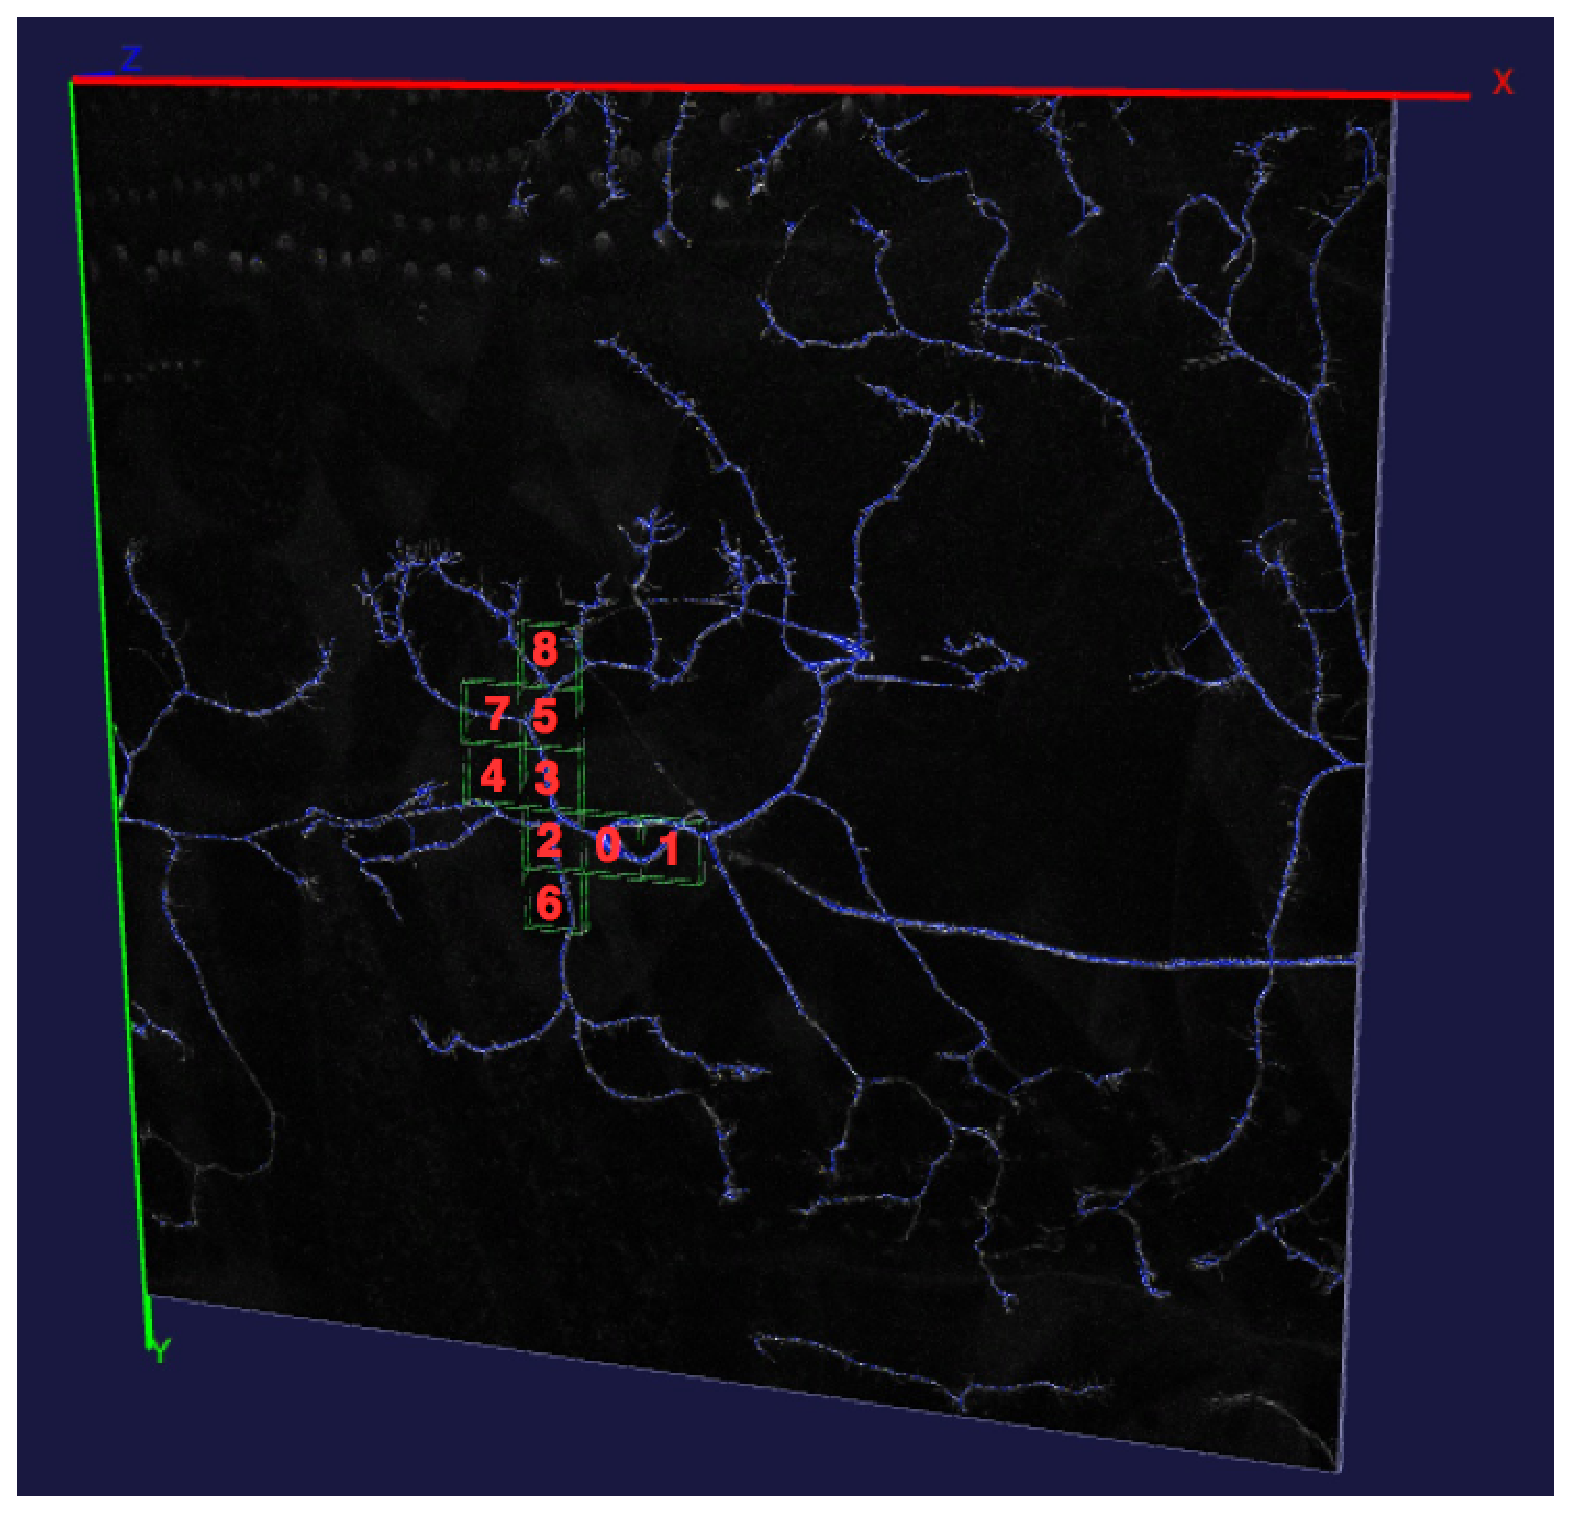
\includegraphics[width=0.29\textwidth,height=0.29\textwidth]{algorithm_illustration/endoftrace.eps}\label{fig:endoftrace}}
    \subfigure[Complete tracing of first 9 blocks.]{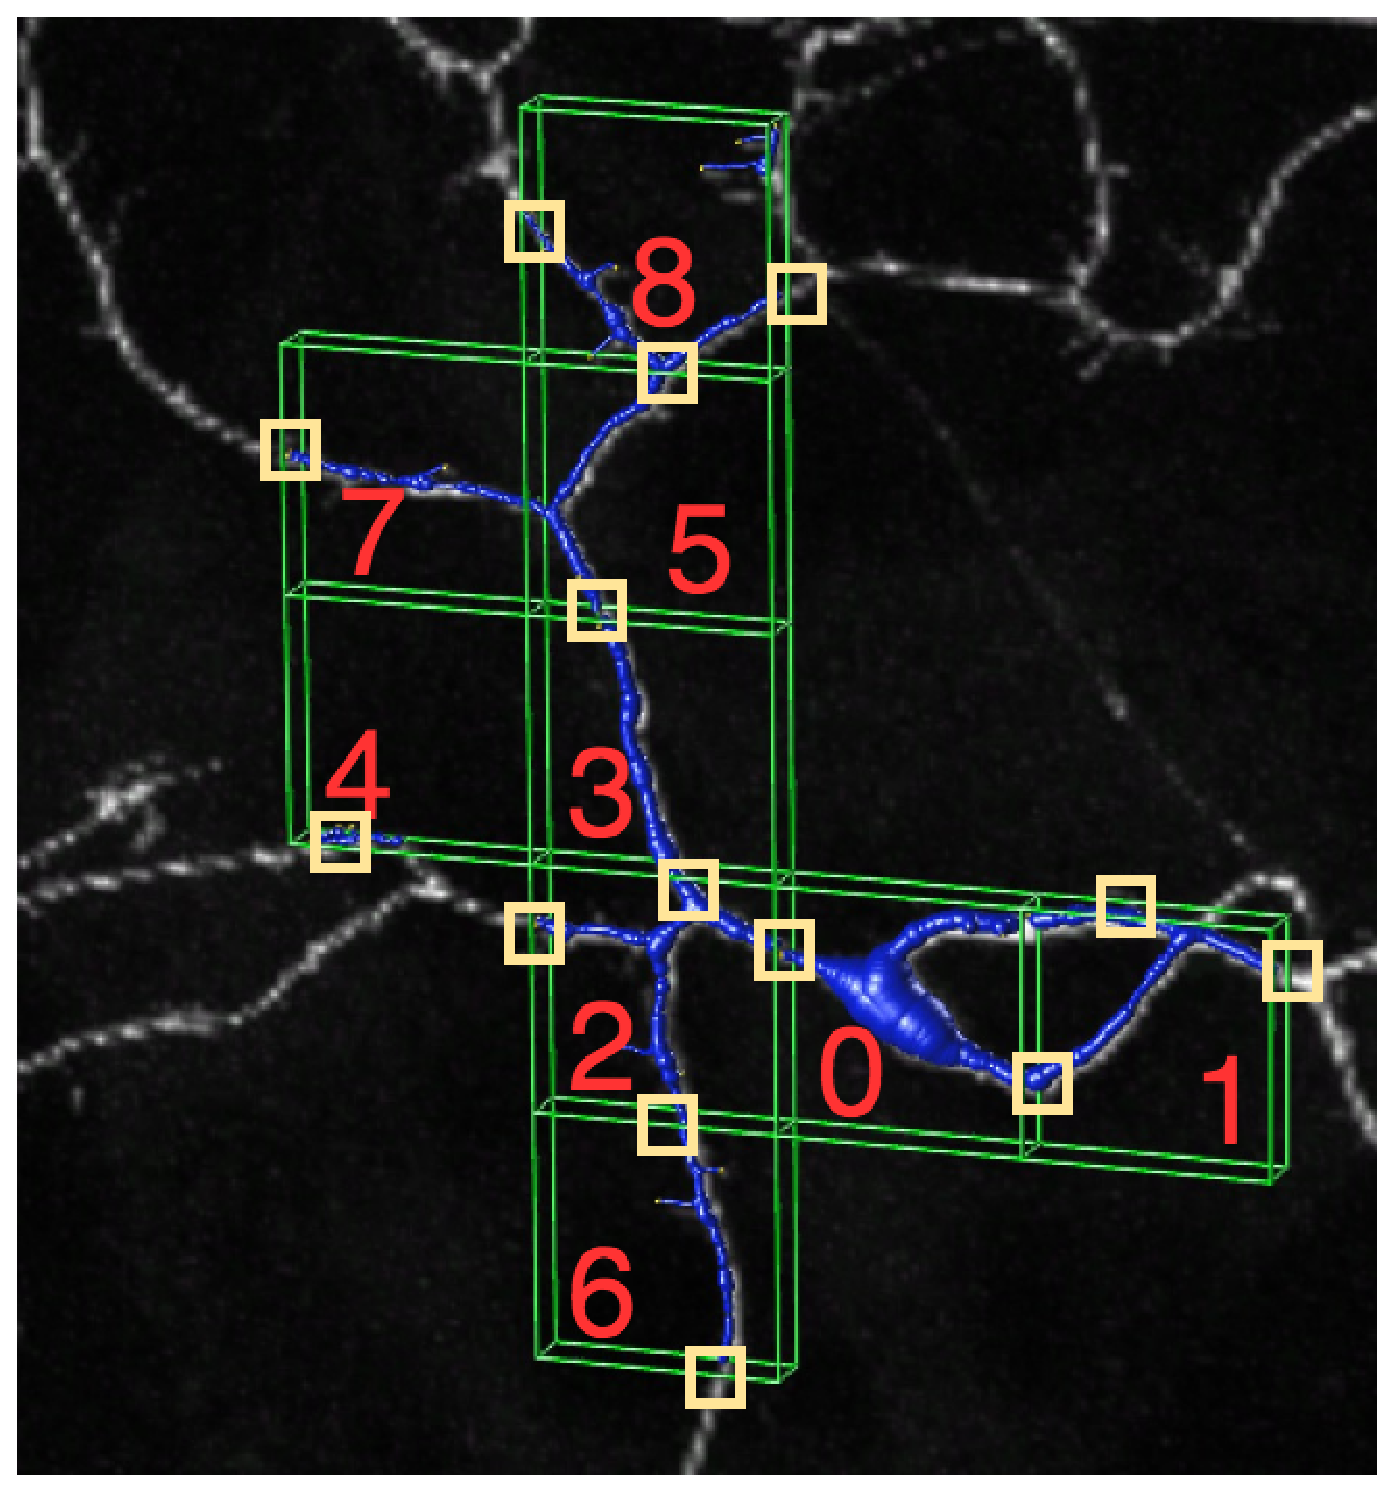
\includegraphics[width=0.29\textwidth,height=0.29\textwidth]{algorithm_illustration/9bk.eps}\label{fig:9bk}}
    \subfigure[Adaptive tracing from one block to the next.]{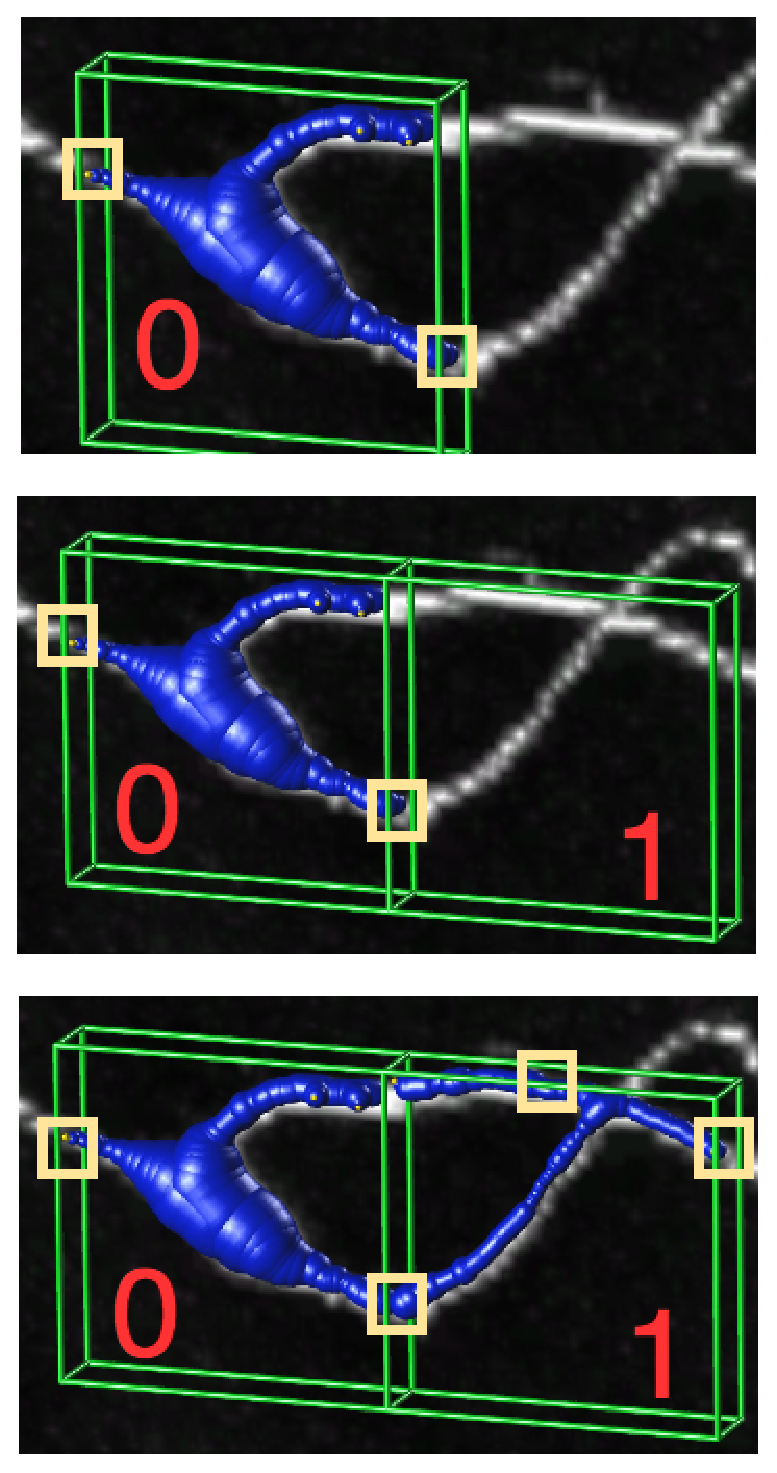
\includegraphics[width=0.16\textwidth,height=0.29\textwidth]{algorithm_illustration/2bk.eps}\label{fig:2bk}}
    \caption{An example of the intermediate steps of adaptive tracing in MEIT.}
    \label{fig:fig1}
\end{figure*}

\section{Related Work}


3D morphology neuron reconstruction algorithms normally involve pre-processing of the raw optical image, detection of the soma position, segmentation of the tree-like structures, and post-processing. Many methods have been proposed to improve the performance of neuron reconstruction by optimizing one or several aspects of the reconstruction algorithm. For example, a method \cite{li2017deep} using Convolutional Neural Networks (CNNs) is applied to pre-process the neuron image. It employs a voxel CNN classifier to get a better estimation of neuron nodes. This classifier learns the discriminative features among different types of neurons and utilizes this knowledge to predict the probability of each voxel in the image belonging to the neuron structures or not. Later, another CNN-based method called Triple-crossing 2.5D CNN \cite{25dcrossingsiqi} was built to enhance the pre-processing accuracy by also identifying disconnected gaps. A few techniques \cite{He2018, Zhang2018soma} were also designed to enhance the soma segmentation process. The soma segmentation method \cite{He2018} automatically detects soma in an efficient way using machine learning techniques. Another method \cite{Zhang2018soma} utilizes a surface evolving algorithm to obtain the soma segmentation inside the soma's estimation bounding box.
 
Our proposed method focuses on improving the efficiency of tree-like architecture segmentation. To successfully trace the complicated morphological neuron structures, many methods \cite{r1_1, r1_2, r2, app, app2, most, rayburst, fm-basu} have been proposed. The Rayburst sampling algorithm  was proposed to perform the radial and volumetric estimation. It estimates the future direction and length of a given node based on the surrounding information of this node. During estimations, it interpolates intensity values continuously between voxels thus leading to the high resolution of structures. More specifically, this sampling algorithm pre-computes a unit array from the given node and samples the image data from multiple directions to get the length which represents the forward distance. Two pruning methods were proposed to improve the accuracy of the tracing algorithm. APP and APP2 initially generate an overtraced reconstruction and run post-processing pruning of unnecessary branches until the coverage of all neuron points reaches a predefined value. To overcome the disadvantages caused by broken structures and background noises, the iterative APP2 alogrithm \cite{tang2017automatic} was proposed. Optimally Oriented Flux (OOF) filter \cite{oof} was used in this method to bridge discontinued connections. MOST \cite{most} extends the previous rayburst sampling algorithm to a marching pattern from seed points. Snake is a method using a 3D open-curve active contour to evolve from automatically detected soma seeds. Its evolution is based on Gradient Vector Flow. 

Whilst APP, APP2, MOST, and Snake start the tracing from soma points and march along neurite branches, Rivulet and Rivulet2 trace from the furthest geometric tips back to soma points or merge to traced branches iteratively. Rivulet iteratively tracks backwards from the likely neuron termini with a confidence score used to decide the possibility of this branch. Rivulet2 further improves the accuracy of Rivulet by erasing traced branches accurately and computing an online confidence score.

It is particularly challenging to trace when the volume of the optical image exceeds a certain value. TreMap \cite{zhou2016tremap} is a new automatic 3D neuron reconstruction algorithm proposed to enhance the effectiveness of reconstruction of large-scale images. This method achieves this advantage by solving the 3D image problem on a 2D plane. It firstly traces the 2D projection of the 3D optical image and then reverses the results back to 3D curves using the 3D virtual finger technique. Then it utilizes the minimal spanning tree method to combine all these curves to generate the final neuron model. Since it performs the tracing method on a 2D plane, it is sufficiently computationally efficient.

\begin{algorithm}
\caption{Our proposed MEIT method}
\label{fmalgorithm}
\begin{algorithmic}[1]
% \resizebox{0.7\linewidth}{!}{
\State \textit{Input}: Initial block $bk_0$, 3D neuron image stack $I$, intensity threshold $t$, adaptive block size $crop_x$ and $crop_y$, traceability threshold $\alpha$, target coverage $\beta$ (the percentage of traced foreground to the whole foreground)
\State \textit{Output}: Tree graph $G$
\State Define $Q$ as an empty queue
\State Define $\overline{bk_i}$ as the percentage of foreground points in ${bk_i}$

\State \textbf{Procedure}
\State Initialize $T(SP(bk_0))$ and $i$ to be 0, store $bk_0$ into $Q$ 
% \State Initialize $Traced(bk_i)$ to be False 
\While{$Q$ is not empty}
\State Extract $bk_{min}$ $\gets$ $argmin$ $T(SP(bk_i))$ in $Q$
\State $bk_i \gets bk_{min}$, $i \gets i + 1$
% \If {$bk_i$ is not traced AND $\overline{bk_i}$\footnotemark{} $\geq \alpha$}
\If {$bk_i$ is not traced AND $\overline{bk_i}$ $\geq \alpha$}

    \State $T_i \gets FM(SP(bk_i), I(bk_i), t)$
    \While{percentage of traced foreground $<$ $\beta$}
    \State Extract $p_{max}$ $\gets$ $argmax$ $T_i$
        \State $branch$ $\gets$ $RK4(p_{max})$
        \If{$Keep(branch)$ is $True$}
            \State Store $branch$ into $G$
            \If{$j$-$th$ face of $bk_0$ touched by $p_{max}$}
                \State $bk_n$ $\gets$ $I(bk_i, crop_x, crop_y, j)$
                \State $SP(bk_n)$ $\gets$ $p_{max}$
                \State $T(SP(bk_n))$ $\gets$ $T(SP(bk_i))+T_i(p_{max})-T_i(SP(bk_i))$
                \State Store $bk_n$ into $Neighbor(bk_i)$
            \EndIf
        \EndIf
    \EndWhile
    \For{any $k$-$th$ face of block $bk_i$ not touched}
        \State $bk_n$ $\gets$ $I(bk_i, crop_x, crop_y, k)$
        \If {$bk_n$ is not traced AND $\overline{bk_n}  > \alpha$}
        \State $SP(bk_n)$ $\gets$ $None$
        \State Store $bk_n$ into $Neighbor(bk_i)$
        \EndIf
    \EndFor
    % \State $Traced(bk_i) \gets True$
    \For{each neighbor $bk$ in $Neighbor(bk_i)$}

        \If {$SP(bk)$ is $None$}
            \State $SP(bk)$ $\gets$ closest point in $B_i$ to $bk_i$
            \State $T(SP(bk))$ $\gets$ $max(T(SP(bk_{adj}))$  $+$ $1$ where all $bk_{adj}$ are in $Neighbour(bk_{i})$ and $SP(bk_{adj})$ is not None 
        \EndIf
        \State Store $bk$ into $Q$
    \EndFor
\EndIf
\EndWhile
\State Return $G$
\end{algorithmic}

\end{algorithm}

Unlike previous work, our method optimizes the reconstruction by using an adaptive tracing algorithm. We start from the initial detected soma area and trace the blocks of the same size around it in an predefined order using the distance transform map. In each block, we start tracing from the center and generate more blocks. This way, we only need to consider a small portion of the image data. During each iteration, we only trace a small block compared to the whole large-scale image, which reduces the memory consumed as well as the computational time.



\section{METHODS}
\label{sec:format}



\subsection{Overview of MEIT}
\label{ssec:overview}
In our method, we take a 3D grey scale image $I(x)$ as the input and trace the image block by block. The initial block is determined based on the soma location (Section \ref{ssec:subhead}), and the subsequent blocks are identified dynamically based on the tracing outputs of the predecessor blocks (Section \ref{ssec:core}). Within each block $bk_i$, a global threshold $t$ is used to get a binary segmentation map $B_i(x)$. Then we generate a 3D boundary distance transform $DT_i(x)$ based on $B_i(x)$. In $DT_i(x)$, voxels that are close to centrelines have larger values while those close to the background have smaller values. A time-crossing map $T_i(x)$ is then generated with the Fast Marching algorithm (FM) \cite{fm-sethian, r1_2} using the speed image $F_i(x)$ generated by $DT_i(x)$. The time-crossing map records the shortest time for each point traveling from the initial location to current position. Detailed explanation is described in Section \ref{ssec:fm}. Each branch is back-tracked iteratively (Iterative Back-tracking, IBT \cite{r2}) based on the gradient of $T_i(x)$ by starting from the geodesic furthest point remaining in the foreground to the source point $SP(bk_i)$. The initial source point $SP(bk_0)$ is detected as the soma point in Section \ref{ssec:subhead}. Later source points are determined by boundary tips of predecessor blocks in Section \ref{ssec:core}. The time-crossing map which is generated with the Fast Marching algorithm (Section \ref{ssec:fm}) is used to decide the order of our tracing. During each iteration of tracing one branch, the next neuron node along the branch is decided by the 4th order Runge-Kutta (Section \ref{ssec:4rk}).


\subsection{Initial Soma Detection}
\label{ssec:subhead}
To detect the soma point of a large-scale optical image efficiently, we downsize $I(x)$ by $\frac{1}{4}$ to $I'(x)$. After applying the same global threshold $t$, the $I'(x)$ is binarized as $B'(x)$. Then we generate a 3D boundary distance transform $DT'(x)$ based on $B'(x)$. The one with greater value in $DT'(x)$ is the one closer to centrelines. Therefore, we take the one with the largest value in $DT'(x)$ as our soma point. With this soma position, we generate a block $bk_0$ centered at the soma point. The size of $xy$-plane of block $bk_0$ is defined by two coefficients $crop_x$ and $crop_y$. This soma point is also the source point $SP(bk_0)$ of this initial block $bk_0$.


\subsection{Large-scale Neuron Reconstruction}
\label{ssec:core}

Instead of directly running FM and IBT on the whole image, after defining the first block $bk_0$, we perform FM and IBT on the current block, then get the source points of neighbouring blocks and again perform FM and IBT on the newly generated block based on the adaptive computation of the time-crossing map.
% in the increasing order of $T(SP(bk_i)$. 

The tracing from one block to the next is illustrated from the top to the bottom of Fig.~\ref{fig:2bk}. We firstly run FM and IBT on the current block $bk_0$. Two endtips marked by yellow frames are detected. 

Next, four neighbouring blocks adjacent to and with the same size as $bk_0$ are generated and we then need to define a source point from which to trace a new block. To maintain the connectivity of the reconstruction, the detected endtips are chosen as the new source points. For boundary faces without endtips, if the block near this boundary face needs to be traced, we define the source point as the foreground point closest to this boundary face. The time-crossing map value of this kind of source point is set to be greater than the maximum among the time-crossing map values of existing source points. In this way, as shown in Fig.~\ref{fig:2bk}, the endtip on the right boundary face has the minimum time-crossing map value. Therefore, the next block to trace is the block adjacent to the right boundary face (i.e. block $1$ in Fig.~\ref{fig:2bk}). Then in $bk_1$, this procedure is repeated and new neighbouring blocks are generated, and the next block to trace is always identified by the source point with minimum time-crossing map value among all existing source points. An example of an adaptive tracing after 9 iterations is shown in Fig.~\ref{fig:9bk}. The detailed steps of the reconstruction are listed in Algorithm \ref{fmalgorithm}. 

The maximum memory consumption occurs when the FM is performed. Traditional FM-based methods \cite{app, app2, r1_2, r2, fm-basu} are performed on the whole image directly whereas our MEIT method only performs FM on a block during each iteration. In addition, only the relative location of the block to the whole image, the values and locations of the time-crossing of the endtips and the traceability of the block are stored rather the time-crossing map of the whole block, which further improves the memory efficiency. 

\subsection{Fast Marching}
\label{ssec:fm}

FM was originally proposed to estimate the path of a moving boundary. The vessel detection method \cite{fm-vu} adapts the original FM to obtain the boundary depth information of a curvilinear structure. Then, APP2 further modifies FM to enhance the intensities of the centerlines of neuronal arbours including dendrites and axons. Unlike original FM, vessel detection method, and APP2, the proposed method follows the design of Rivulet and Rivulet2, using FM to generate the time-crossing map. With the obtained time-crossing map, each step of MEIT follows its gradient information. The gradient information is smoothly estimated using the 4th Order Runge-Kutta method to avoid trapping the tracing in the highly discontinuous neuronal arbours discussed in the following section.          

Time-crossing map $T$ is obtained by solving the following Eq.~(\ref{eq:fm}): 
\begin{eqnarray}
\vspace{-0.4cm}
F = \frac{dx}{dT},\quad |\nabla{T}|F = 1, \quad T(\Gamma_{0}) = 0 
\label{eq:fm}
\end{eqnarray}
where $F$ is the evolution speed and $\Gamma_{0}$ is the initial condition~\cite{adalsteinsson1995fast}.

Then, the value of the time-crossing map at each discrete point which is further simplified as the shortest time of traveling from source point (usually soma location) is defined as:  
\begin{eqnarray}
T(x) = \min_{P_{(s, x)}} \int_{0}^{L} C(P(t))dt \\
C(P(t)) = {\left(\frac{F(P(t))}{\max{F}}\right)}^{4} 
\label{eq:timecross}
\end{eqnarray}
where $P_{(s, x)}$ are possible paths $L$ from the starting point $s$ to $x$. $C(.)$ is the cost function to ensure the centerline has a higher evolution speed than the boundary of the curvilinear structure.  

\subsection{4th Order Runge-Kutta of Gradient Estimation}
\label{ssec:4rk}

Our proposed MEIT method is able to identify the direction of the next move by manipulating the subvoxel gradient with Runge-Kutta \cite{r1_2} defined as: 
\begin{equation}
\begin{cases}
k_1 = 0.5\alpha / max(\|\nabla T(p_i)\|, 1)\\
p_{i,1} = p_i - k_1\\
k_2 = 0.5\alpha / max(\|\nabla T(p_{i,1})\|, 1)\\
p_{i,2} = p_{i,1} - k_2\\
k_3 = \alpha / max(\|\nabla T(p_{i,2})\|, 1)\\
p_{i,3} = p_{i,2} - k_3\\
k_4 = \alpha / max(\|\nabla T(p_{i,3})\|, 1)\\
p_{i+1} = p_i - (k_1 + 2k_2 + 2k_3 + k_4)/6
\end{cases}
\label{RK4}
\end{equation}
where $k_1,k_2,k_3,k_4$ are the direction vectors at the corresponding point $p$, and $\alpha$ is a constant set to $1$ in our experiment. A special case is applied to prevent the tracing from trapping at a local minimal, for which the momentum~\cite{r2} update rule is defined as: 
\begin{equation}
p_{i+1} = 2p_i - p_{i-2}~~\text{if}~\|p_{i+1} - p_i\|_2^2 ~\text{is small}
\end{equation}



\begin{figure*}[htb]
\centering
    \subfigure[Peak computer memory consumed when processing relatively large images for each species using Rivulet2 and MEIT.]{\includegraphics[width=0.4\textwidth]{mem_v7.eps}\label{fig:memory}}
    \subfigure[Peak reconstruction time consumed when processing relatively large images for each species using Rivulet2 and MEIT.]{\includegraphics[width=0.4\textwidth, height=0.27\textwidth]{time_compare_v2.eps}\label{fig:reconstruction_time}}
    \subfigure[The precision results of Gold dataset generated by MEIT and compared methods.]{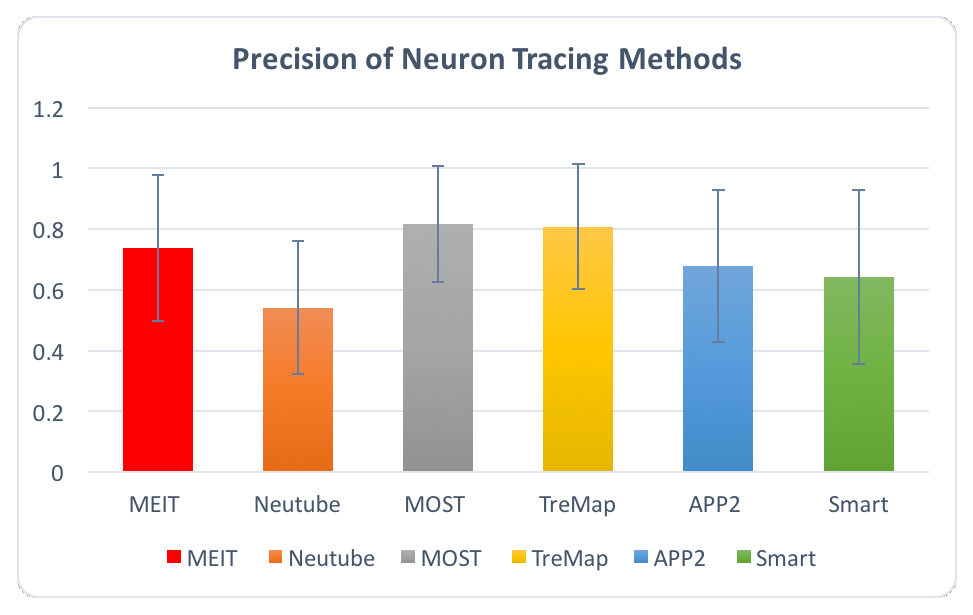
\includegraphics[width=0.4\textwidth]{precision.eps}\label{fig:precision}}
    \subfigure[The recall results of Gold dataset generated by MEIT and compared methods.]{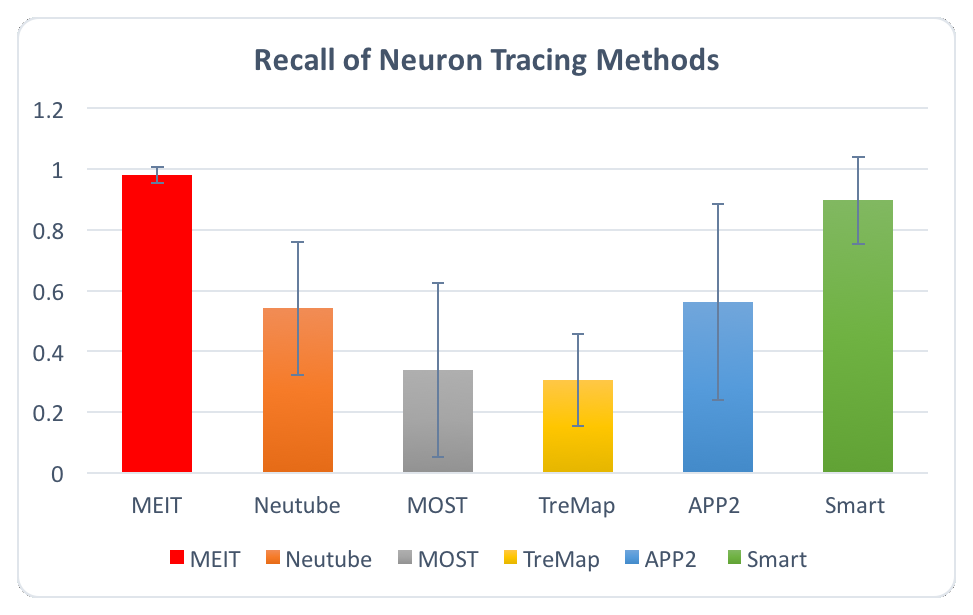
\includegraphics[width=0.4\textwidth]{recall.eps}\label{fig:recall}}
    \subfigure[The F1-score results of Gold dataset generated by MEIT and compared methods.]{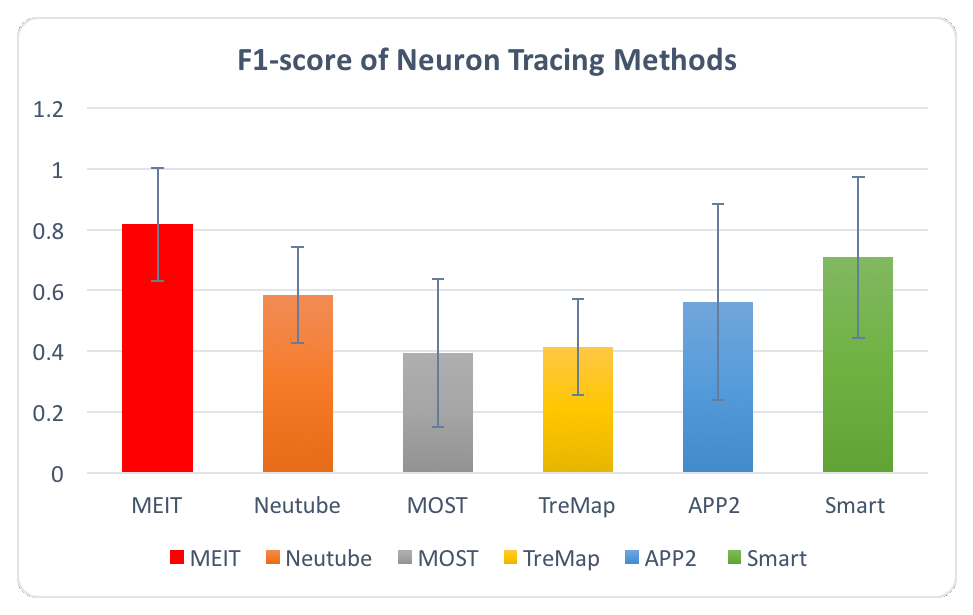
\includegraphics[width=0.4\textwidth]{f1_score.eps}\label{fig:accuracy}}
    \subfigure[The number of successful neuron reconstructions generated by the proposed method and compared methods with 156 neuron images from fruitfly larvae to human.]{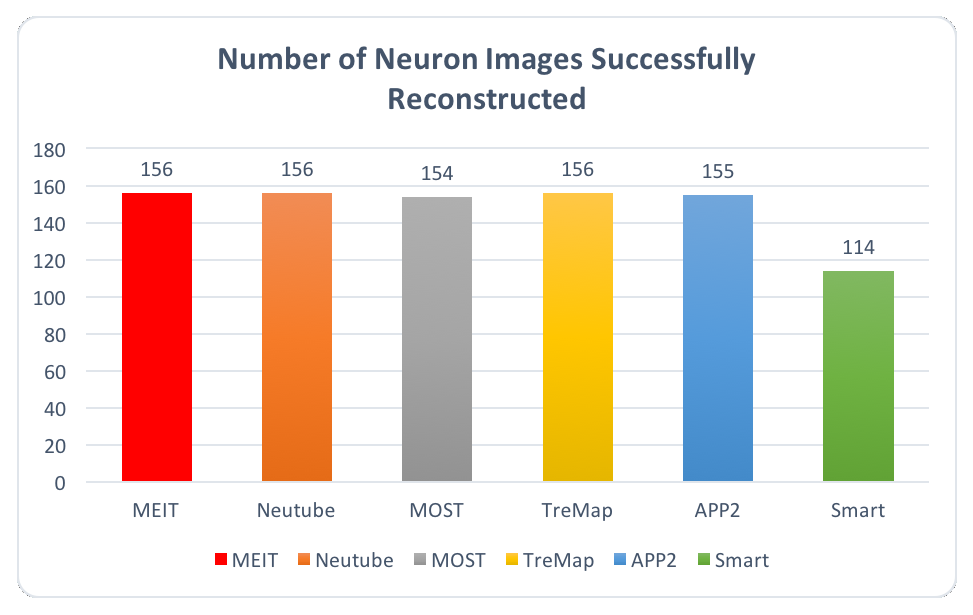
\includegraphics[width=0.4\textwidth]{number.eps}\label{fig:reconstruction_number}} 
    
        \caption{Comparison with state-of-the-art methods.}
    \label{fig:mem_time}
\end{figure*}


\begin{figure*}[!ht]
\centering
\subfigure[The reconstruction of a fly neuron image.]{
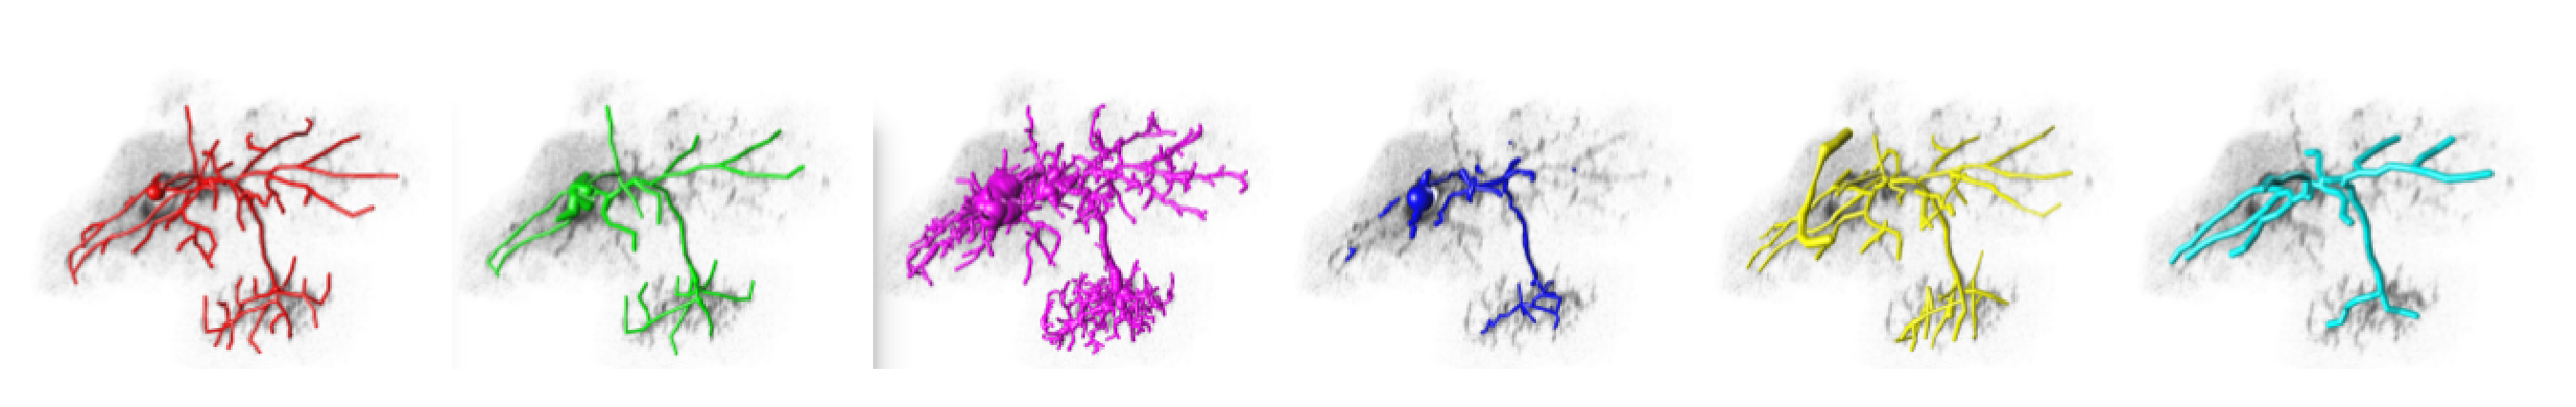
\includegraphics[width=0.85\textwidth, height=0.12\textwidth]{methods_1.eps}\label{fig:fly}
}
\subfigure[The reconstruction of a human neuron image.]{
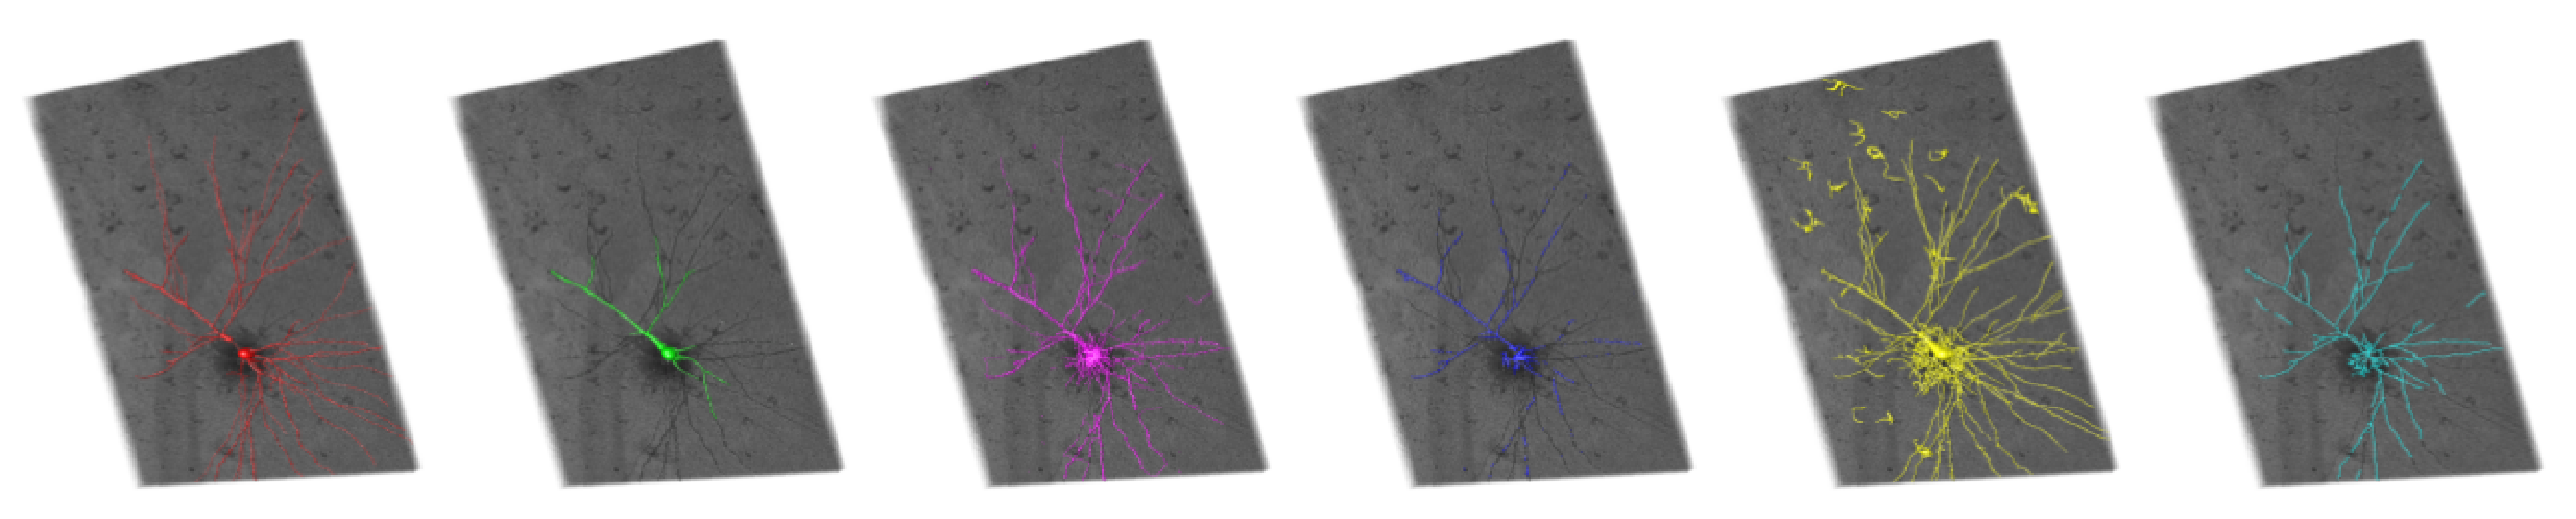
\includegraphics[width=0.85\textwidth, height=0.17\textwidth]{methods_2.eps}\label{fig:human}
}
\subfigure[The reconstruction of a mouse neuron image.]{
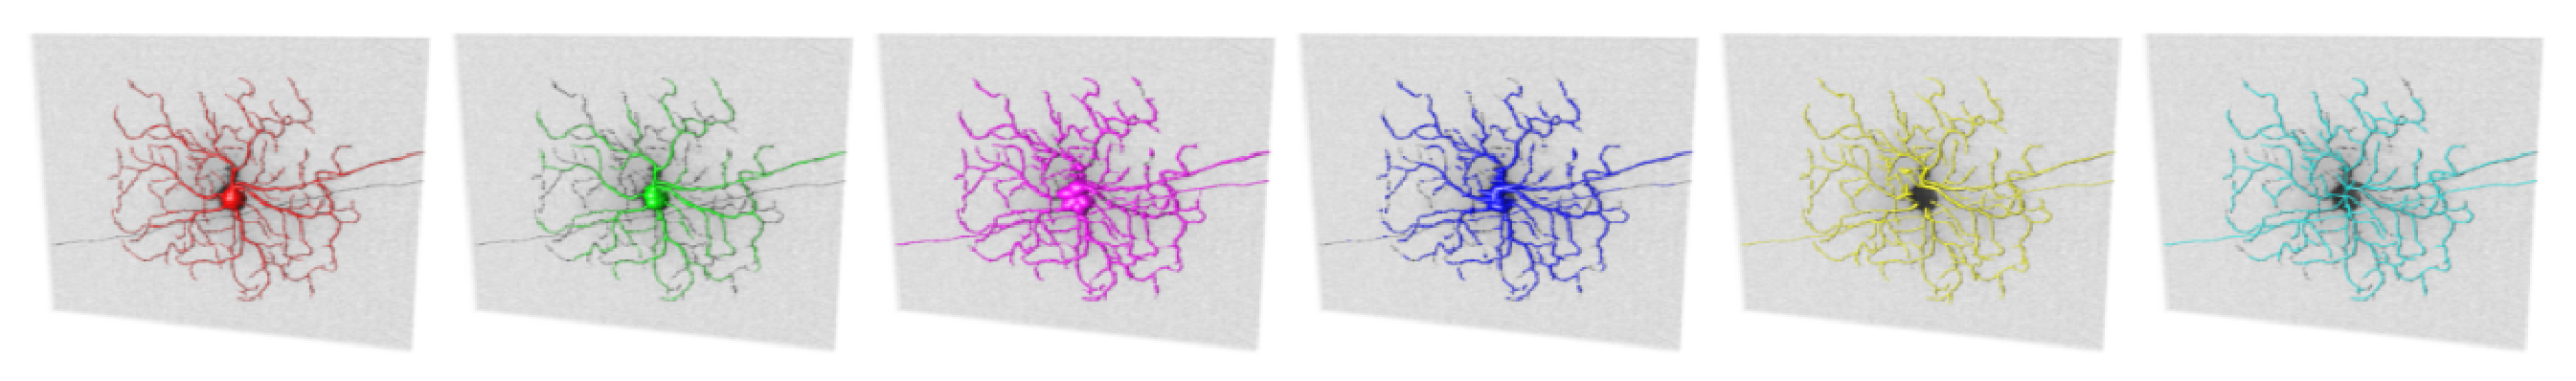
\includegraphics[width=0.85\textwidth, height=0.12\textwidth]{methods_3.eps}\label{fig:mouse}
}
\subfigure[The reconstruction of a silkmoth neuron image.]{
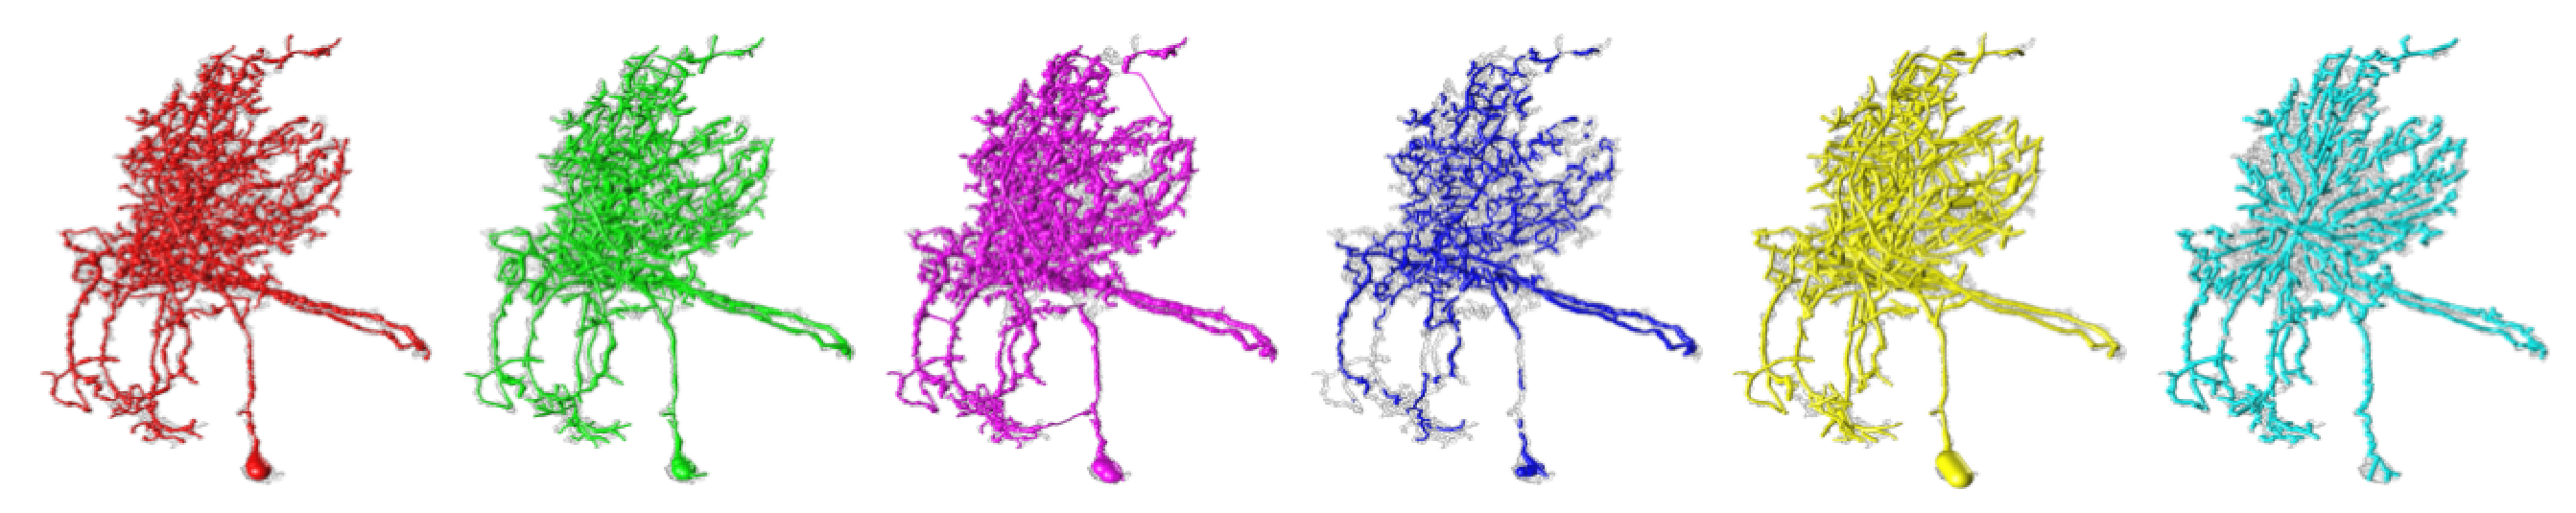
\includegraphics[width=0.85\textwidth, height=0.17\textwidth]{methods_4.eps}\label{fig:silkmoth}
}
\subfigure[The reconstruction of a zebrafish neuron image.]{
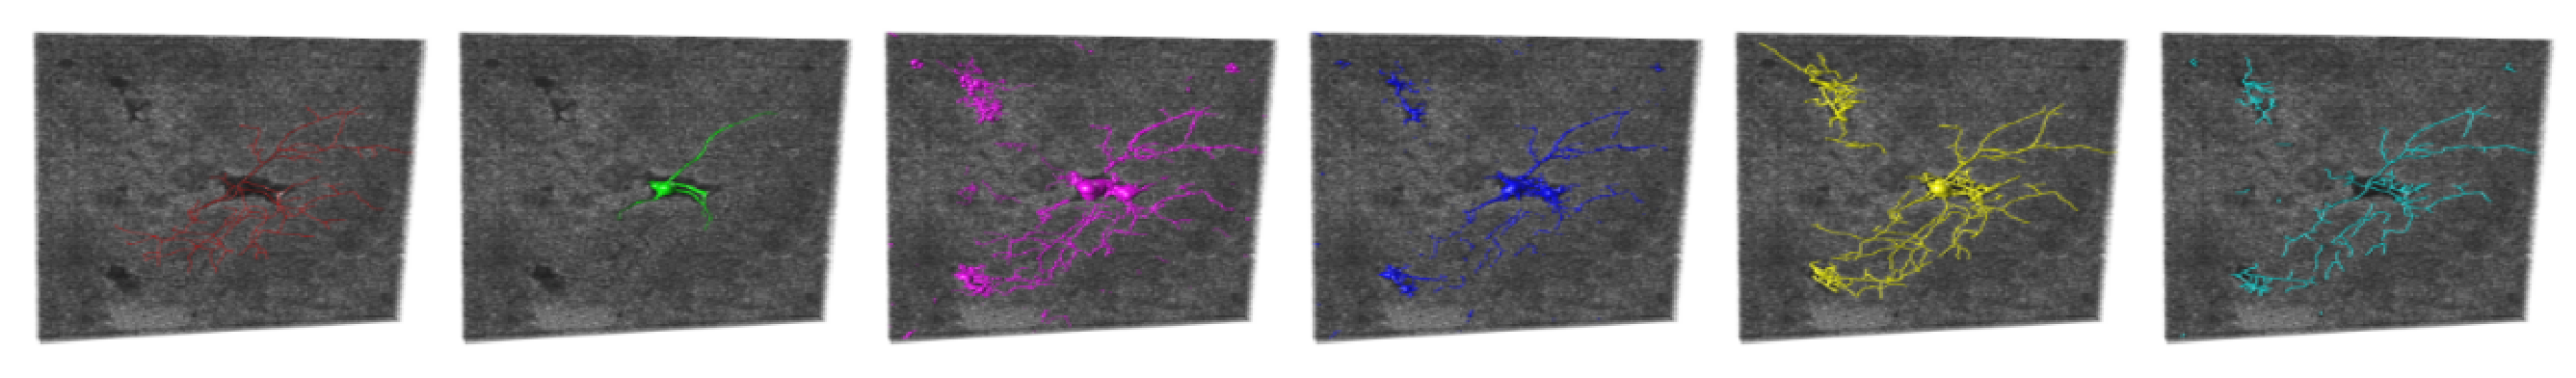
\includegraphics[width=0.85\textwidth, height=0.12\textwidth]{methods_5.eps}\label{fig:zebrafish}
}
\subfigure[The reconstruction of a chick neuron image.]{
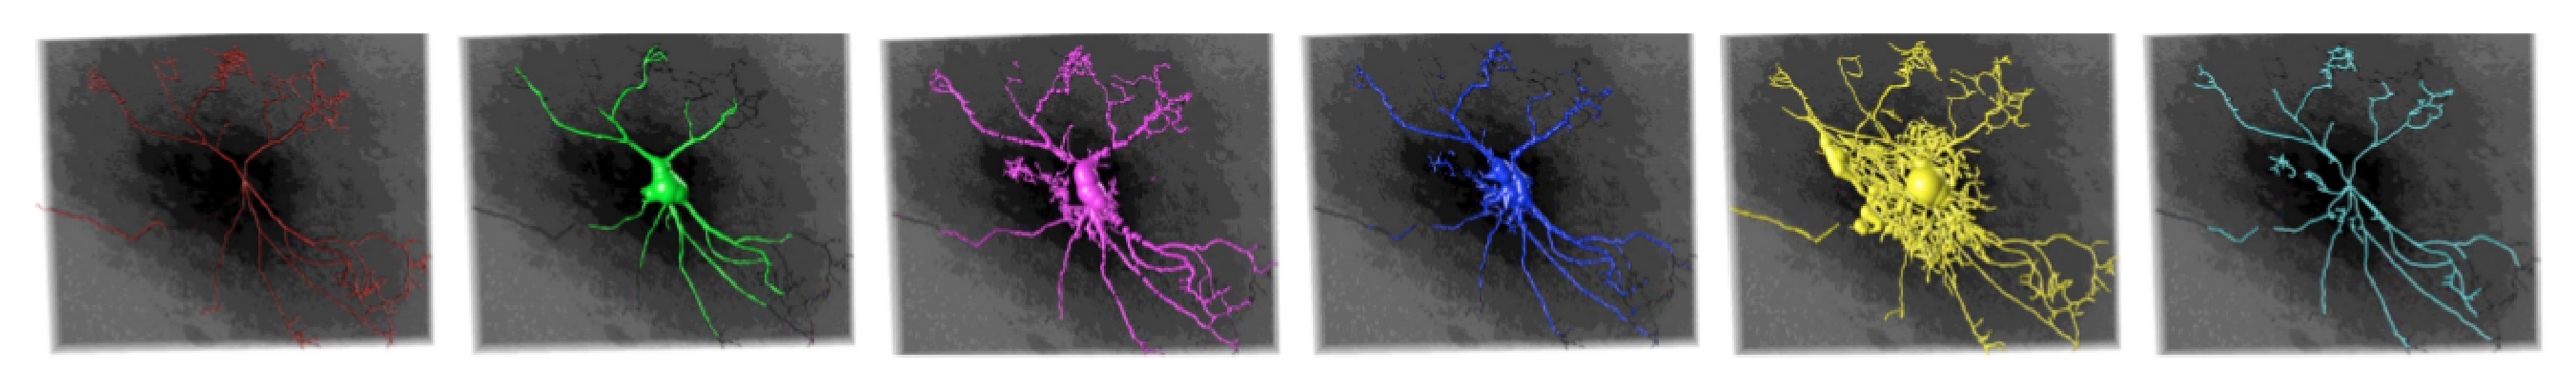
\includegraphics[width=0.85\textwidth, height=0.12\textwidth]{methods_6.eps}\label{fig:chick}
}
\subfigure[The reconstruction of a fruit fly larvae neuron image.]{
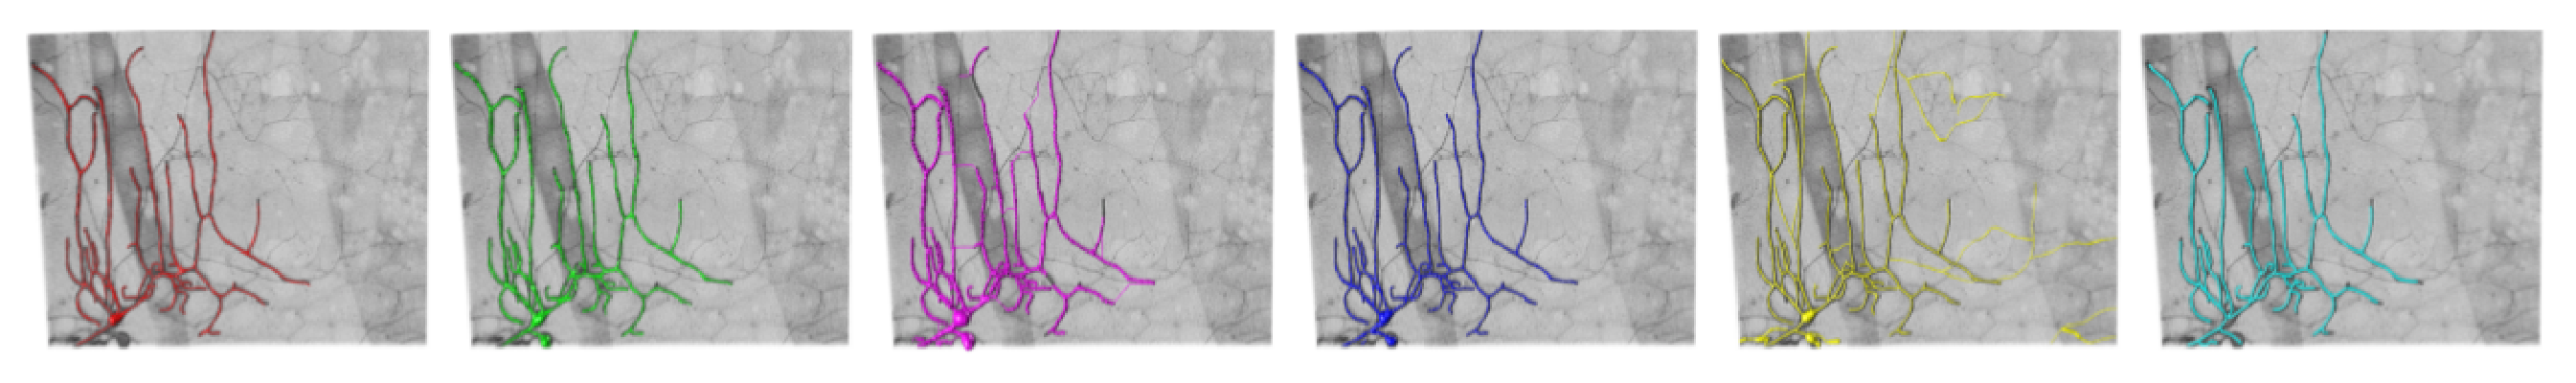
\includegraphics[width=0.85\textwidth, height=0.12\textwidth]{methods_7.eps}\label{fig:larvae}
}
{\begin{tabu} to 0.9\textwidth {X[c]  X[c]  X[c]  X[c] X[c] X[c]}
\textbf{Ground Truth} & \textbf{APP2} & \textbf{MEIT} & \textbf{MOST} & \textbf{Neutube}  & \textbf{TreMap}   
\end{tabu}}
\caption{The comparison between our proposed method and four other state-of-the-art algorithms on neuron reconstruction result.} 

\label{fig:methods}
\end{figure*}






\section{Experiment}
\label{sec:experiment}
\subsection{Dataset and Setup}
We evaluated our method on the Gold dataset from the BigNeuron project which contains 156 3D neuron images. We provided a Python implementation of MEIT\footnote{https://github.com/wkkxixi/MEIT}. These images belong to 8 species categories, including mouse, silkmoth, human, zebrafish, fruitfly larvae, chick, fly, and frog. Each neuron image in this dataset has a corresponding ground truth of neuron reconstruction labelled by computational neuroscientists. The number of voxels of these 3D images varies from 632520 to 629145600 voxels. 
% The results of the neuron reconstruction are visualized by Vaa3D~\cite{v3d}. 
We set the traceability threshold $\alpha$ and the target coverage $\beta$ to be 0.00005 and 0.98 respectively. The cropping parameters $crop_x$ and $crop_y$ are both set to be 100. The setting of threshold $t$  is adaptive to individual images and follows the technique used in Rivulet2.

\subsection{Neuron Reconstruction Accuracy}
\label{sec:v-q-compare}
Three methods were evaluated in our quantitative comparison, including the state-of-the-art method Rivulet2 \cite{r2}, naive cropping of Rivulet2 (Crop), and our MEIT method.  Crop divides a neuron image into blocks with same size and simply applies Rivulet2 as a base tracer for each block without considering the orders of the neuronal tree structure. Finally, these individual reconstructions are combined together to obtain the reconstruction of the whole image. MEIT, compared to Crop, does not divide the image before the tracing, instead tracing the image adaptively by considering the value of the time-crossing map of FM during the reconstruction.  

\begin{table}[htbp]
\caption{The quantitative comparison between Rivulet2, Crop and MEIT. The number beside the dataset name is the number of 3D images in each dataset. The number of the successful reconstructions are shown beside the method name.}
\begin{center}
\begin{tabular}{|l|l|l|l|}
\hline
fruitfly larvae 12& Precision         & Recall             & F1      \\
\hline
Rivulet2 (12/12)    & $\textbf{0.617}$ $\boldsymbol{\pm}$ $\textbf{0.147}$   & $0.902\pm0.105$  & $0.722\pm0.117$\\
Crop (12/12) & $0.547\pm0.129$   & $0.951\pm0.057$  &  $0.684\pm0.111$\\
proposed (12/12) & $0.599\pm0.127$   & $\textbf{0.983}$ $\boldsymbol{\pm}$ $\textbf{0.026}$  &  $\textbf{0.736}$ $\boldsymbol{\pm}$ $\textbf{0.100}$\\ 
\hline
fly 79 &\multicolumn{3}{l|}{}\\
\hline
Rivulet2 (79/79)    & $\textbf{0.925}$ $\boldsymbol{\pm}$ $\textbf{0.105}$   & $0.908\pm0.076$  & $0.912\pm0.084$\\
Crop (79/79) & $0.869\pm0.147$   & $0.962\pm0.047$  &  $0.905\pm0.108$\\
proposed (79/79) & $0.911\pm0.102$   & $\textbf{0.987}$ $\boldsymbol{\pm}$ $\textbf{0.023}$  &  $\textbf{0.944}$ $\boldsymbol{\pm}$ $\textbf{0.065}$\\
\hline
zebrafish 13 &\multicolumn{3}{l|}{}\\
\hline
Rivulet2 (13/13)    & $0.587\pm0.176$   & $0.911\pm0.052$  & $0.698\pm0.147$\\
Crop (13/13) & $0.471\pm0.146$   & $0.927\pm0.025$  &  $0.611\pm0.136$\\
proposed (13/13) & $\textbf{0.588}$ $\boldsymbol{\pm}$ $\textbf{0.137}$   & $\textbf{0.983}$ $\boldsymbol{\pm}$ $\textbf{0.009}$  & $\textbf{0.725}$ $\boldsymbol{\pm}$ $\textbf{0.118}$\\ 
\hline
silkmoth 7 &\multicolumn{3}{l|}{}\\
\hline
Rivulet2 (7/7)    & $\textbf{0.877}$ $\boldsymbol{\pm}$ $\textbf{0.078}$   & $0.916\pm0.119$  & $0.890\pm0.080$\\
Crop (7/7) & $0.814\pm0.067$   & $0.946\pm0.061$  &  $0.874\pm0.044$\\
proposed (7/7) & $0.876\pm0.039$   & $\textbf{0.989}$ $\boldsymbol{\pm}$ $\textbf{0.013}$  &  $\textbf{0.929}$ $\boldsymbol{\pm}$ $\textbf{0.023}$\\ 
\hline
frog 1 &\multicolumn{3}{l|}{}\\
\hline
Rivulet2 (1/1)    & $0.670\pm0.000$   & $0.970\pm0.000$  & $0.790\pm0.000$\\
Crop (1/1) & $0.610\pm0.000$   & $0.970\pm0.000$  &  $0.750\pm0.000$\\
proposed (1/1) & $\textbf{0.810}$$\pm$$\textbf{0.000}$   & $\textbf{1.000}$ $\boldsymbol{\pm}$ $\textbf{0.000}$  &  $\textbf{0.890}$ $\boldsymbol{\pm}$ $\textbf{0.000}$\\ 
\hline
mouse 29 &\multicolumn{3}{l|}{}\\
\hline
Rivulet2 (28/29)    & $\textbf{0.607}$ $\boldsymbol{\pm}$ $\textbf{0.169}$   & $0.889 \pm 0.066$  & $\textbf{0.706}$ $\boldsymbol{\pm}$ $\textbf{0.141}$\\
Crop (29/29) & $0.477\pm0.188$   & $0.936\pm0.067$  &  $0.608\pm0.168$\\
proposed (29/29) & $0.480\pm0.186$   & $\textbf{0.981}$ $\boldsymbol{\pm}$ $\textbf{0.020}$  &  $0.624\pm0.166$\\ 
\hline
chick 8 &\multicolumn{3}{l|}{}\\ 
\hline
Rivulet2 (8/8)    & $\textbf{0.414}$ $\boldsymbol{\pm}$ $\textbf{0.204}$   & $0.781\pm0.124$  & $\textbf{0.525}$ $\boldsymbol{\pm}$ $\textbf{0.208}$\\
Crop (8/8) & $0.378\pm0.198$   & $0.813\pm0.114$  &  $0.495\pm0.205$\\
proposed (8/8) & $0.333\pm0.172$   & $\textbf{0.935}$ $\boldsymbol{\pm}$ $\textbf{0.048}$  &  $0.470\pm0.194$\\ 
\hline
human 7 &\multicolumn{3}{l|}{}\\ 
\hline
Rivulet2 (7/7)    & $\textbf{0.824}$ $\boldsymbol{\pm}$ $\textbf{0.108}$   & $0.891\pm0.094$  & $\textbf{0.851}$ $\boldsymbol{\pm}$ $\textbf{0.079}$\\
Crop (7/7) & $0.710\pm0.144$   & $0.929\pm0.041$  &  $0.797\pm0.104$\\
proposed (7/7) & $0.707\pm0.193$   & $\textbf{0.966}$ $\boldsymbol{\pm}$ $\textbf{0.032}$  &  $0.804\pm0.133$\\
\hline
\end{tabular}
\label{tab:quant}
\end{center}
\end{table}



Table \ref{tab:quant} shows the quantitative results using precision, recall and F1-score. The result shows that MEIT outperforms Rivulet2 in term of F1-scores in fruitfly, fly, silkmoth, zebrafish, and frog. The reason is that MEIT traces block-by-block rather than tracing the whole image, and, in this way, FM can depict more details of the neuronal tree structure. Instead of detailed branch cut of Rivulet2, our proposed method implements a more efficient block traceability determination but can be less accurate, which results in lower precision in some cases. The higher recalls of our method compared to Rivulet2 is due to errors of fast marching introduced by gaps or discontinuities of neuronal structure not accumulative, and source point finding strategy of blocks without endtips on the boundary face.             
\subsection{Peak Memory and Time Consumption}

Our goal is to show that the proposed method is not only accurate (shown in Section \ref{sec:v-q-compare}) but also memory-efficient as well as time-saving when tracing a neuron image with ultra-volume. Our method performs tracing at the block level during each iteration while in Rivulet2 it traces a whole large image directly and creates the time-crossing map of the whole neuronal structure. Therefore, our method stands out when the image is quite large. 

To demonstrate that our method is efficient in memory and time, we compared the peak memory as well as time consumed when performing Rivulet2 \cite{r2} and our proposed method on relatively large neuron images from eight different species. The result in Fig.~\ref{fig:memory} shows that the consumed memory of MEIT is less than $\frac{1}{7}$ of the memory used by Rivulet2 except for the frog example in which MEIT consumed just under $\frac{1}{4}$ of the memory used by Rivulet2. 

The main processing time spent during the process of Rivulet2 was on the tracing of the main neuron structure. During each iteration, Rivulet2 scans the whole image which takes unnecessary time and memory. Since we only run the fast marching algorithm on a small portion of the original image each iteration, the efficiency is enhanced a great deal. As shown in Fig.~\ref{fig:reconstruction_time}, MEIT requires extensively less running time than Rivulet2. 

\subsection{Comparison with Existing Methods}
We quantitatively compared our method MEIT with several other state-of-the-art methods which include Neutube \cite{neutube}, MOST \cite{most}, TreMap \cite{zhou2016tremap}, APP2 \cite{app2}, and Smart \cite{smarttracing}. We computed the precision, recall, and F1-score of each method when comparing their reconstruction result of the neuron images from the Gold dataset. As shown in Fig.~\ref{fig:precision} and Fig.~\ref{fig:recall}, MEIT achieves the average precision and highest recall among these methods. This demonstrates that our proposed method detects the largest number of neuron nodes among these state-of-the-art algorithms. This advantage is particularly noticeable when there are disconnected fibres in the original neuron image. Furthermore, as indicated in Fig.~\ref{fig:accuracy}, MEIT reaches the highest F1-score among these techniques, demonstrating the overall advantage of our method.

It can also be seen that some methods such as MOST, APP2, and Smart are constrained by the type of species. Fig.~\ref{fig:reconstruction_number} shows that MEIT, Neutube, and TreMap successfully reconstructed all neuron images used in the Gold dataset. This demonstrates that our method can tackle various types of neurons like the other state-of-the-art algorithms.

Fig.~\ref{fig:methods} shows some reconstruction results comparing the various methods. In the reconstruction of the fly neuron image and the zebrafish neuron image, as shown in Fig.~\ref{fig:fly} and Fig.~\ref{fig:zebrafish}, MEIT can trace the whole neuron structure even though there are many small gaps around it. The human neuron image in the second row as well as the fruit fly larvae neuron image in the last row are contaminated with background noise. As indicated by Fig.~\ref{fig:human} and Fig.~\ref{fig:larvae}, our proposed method was not affected by the noise and traced the neuron structure successfully. Fig.~\ref{fig:silkmoth} and Fig.~\ref{fig:zebrafish} display the reconstruction of three complicated neuron images. It can be seen that MEIT achieved almost the same effect as the other state-of-the-art methods when the neuron image is complicated with our less laborious and more memory-efficient algorithm. The chick neuron image in Fig.~\ref{fig:chick} contains unevenly distributed intensity. Our proposed method MEIT outperformed the Neutube method in such a situation. 




\section{Conclusion}
Reconstruction of the intensively large neuron image typically requires a massive amount of memory and time. To solve this problem, our MEIT method traces an image adaptively by tracing only a small block of the whole image during each iteration based on the minimum time-crossing map value of endtips from each traced block. The proposed method was evaluated on the Gold dataset provided by the BigNeuron project. The results showed that our method achieves overall better reconstruction performance than those state-of-the-art methods and requires significantly less memory and time.



\bibliographystyle{IEEEbib}
\bibliography{refs.bib}

\end{document}

\section*{References}

